\documentclass[11pt]{article}

\usepackage[a4paper,margin=1in]{geometry}
\usepackage{amsmath,amssymb,amsthm,mathtools}
\usepackage{graphicx}
\usepackage{microtype}
\usepackage{xcolor}
\usepackage{enumitem}
\usepackage[hidelinks]{hyperref}

\definecolor{statusblue}{RGB}{32,78,121}
\newtheorem{theorem}{Theorem}
\newtheorem{lemma}{Lemma}
\newcommand{\D}{\mathbb D}
\newcommand{\T}{\mathbb T}
\newcommand{\dd}{\,d}
\newcommand{\norm}[1]{\left\lVert#1\right\rVert}

\title{\textbf{General \(L^2\) Poisson Concentration}\\
\large A sharp uniform-factor answer to Remark 5 of arXiv:2411.16010}
\author{Automated mathematics run \texttt{fa\_banach\_001}\\
Lane 14, model GPT5.6}
\date{23 July 2026}

\begin{document}
\maketitle

\begin{abstract}
Gómez, Kalaj, Melentijević, and Ramos ask whether their sharp concentration
inequality for analytic Hardy functions has an analogue for Poisson
extensions of arbitrary \(L^2\) boundary data. We give an affirmative answer
with multiplicative factor \(2\), prove that \(2\) is the best factor uniform
in the hyperbolic area, and show that the analytic sharp factor \(1\) fails
for every fixed positive area. The upper bound is the analytic/anti-analytic
splitting. Sharpness is forced by normalized Poisson kernels whose centers
approach the boundary.
\end{abstract}

\noindent
\colorbox{statusblue!10}{\parbox{0.96\linewidth}{
\textbf{Status.} Candidate full result; verifier verdict: likely valid.
Human review is recommended, especially for normalization and novelty.
The result determines the best factor uniform over all \(s>0\), not the
fixed-\(s\) optimal constant.
}}

\section{Source question}

The source is Gómez--Kalaj--Melentijević--Ramos,
\emph{Uniform stability of concentration inequalities and applications},
arXiv:2411.16010 \cite{GKMR}. Their Theorem 1.4 contains the qualitative
inequality
\begin{equation}\label{eq:analytic}
 \int_\Omega |f(z)|^2(1-|z|^2)^{-1}\dd A(z)
 \le
 \pi\log\!\left(1+\frac{s}{\pi}\right)\norm{f}_{H^2}^2,
 \qquad f\in H^2(\D),
\end{equation}
where
\[
 d\mu(z)=(1-|z|^2)^{-2}\dd A(z),
 \qquad \mu(\Omega)=s.
\]
Remark 5 on pp.~41--42 then asks:
\begin{quote}
\emph{Can one obtain a concentration inequality for Poisson extensions of
general \(L^2\) functions on the boundary of the unit disk?}
\end{quote}

\begin{figure}[ht]
\centering
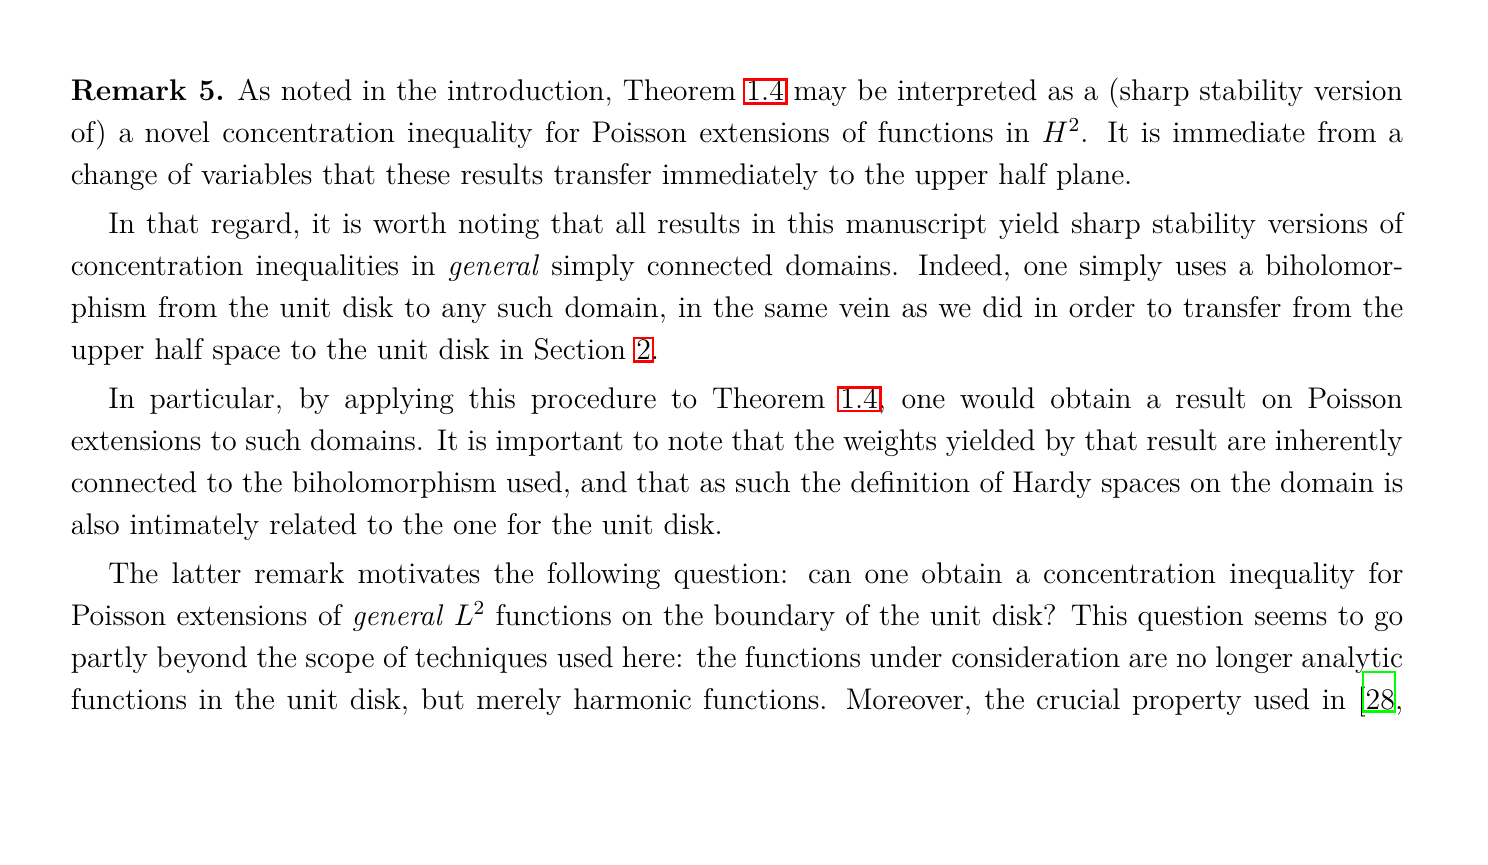
\includegraphics[width=\textwidth]{figures/open_problem_crop_page41.png}
\vspace{0.4em}
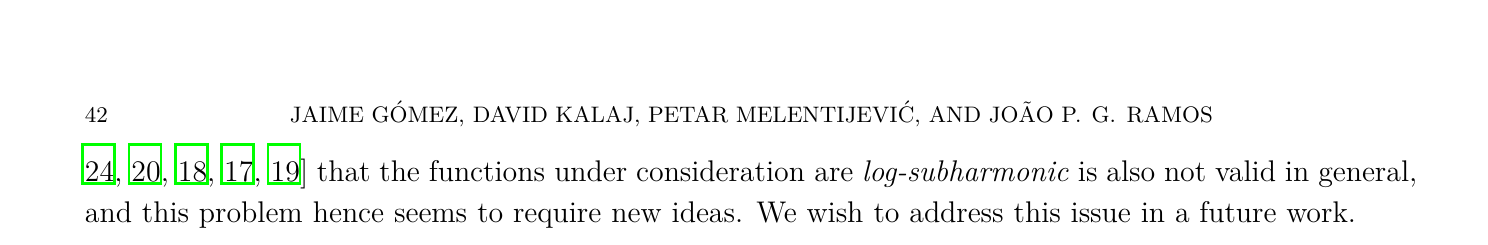
\includegraphics[width=\textwidth]{figures/open_problem_crop_page42.png}
\caption{The complete source question, spanning pp.~41--42 of
arXiv:2411.16010.}
\end{figure}

\section{Normalization and proof intuition}

Give \(\T\) normalized measure
\[
 dm(e^{it})=\frac{\dd t}{2\pi}.
\]
If
\[
 h(e^{it})=\sum_{n\in\mathbb Z}a_ne^{int}\in L^2(\T,dm),
\]
its Poisson extension is
\[
 u(re^{it})=P[h](re^{it})
 =\sum_{n\in\mathbb Z}a_nr^{|n|}e^{int}.
\]

\paragraph{Proof intuition.}
The obstruction noted in the source is the failure of log-subharmonicity for
a general harmonic function. There is no need to restore it. The positive and
negative Fourier halves of \(u\) are separately analytic, so the source
inequality applies to each half. Their interference costs at most a factor
\(2\).

That loss is genuinely necessary in a uniform theorem. A normalized boundary
Poisson kernel has nearly equal analytic and anti-analytic halves. Moving its
center and a fixed pseudohyperbolic disk together toward the boundary makes
the two halves reinforce. The pullback to a fixed Euclidean disk leaves one
elementary angular integral, from which both the failure of factor \(1\) and
the sharpness of factor \(2\) follow.

\section{Main theorem}

\begin{theorem}\label{thm:main}
Let \(h\in L^2(\T,dm)\), let \(u=P[h]\), and let
\(\Omega\subset\D\) be measurable with \(\mu(\Omega)=s<\infty\). Then
\begin{equation}\label{eq:main}
 \int_\Omega |u(z)|^2(1-|z|^2)^{-1}\dd A(z)
 \le
 2\pi\log\!\left(1+\frac{s}{\pi}\right)\norm{h}_2^2.
\end{equation}
The factor \(2\) is the least constant which can replace it uniformly for all
\(s>0\). Moreover, the corresponding inequality with factor \(1\) fails for
every fixed \(s>0\).
\end{theorem}

\subsection{Upper bound}

\begin{proof}[Proof of \eqref{eq:main}]
Define
\[
 f(z)=\sum_{n\ge0}a_nz^n,
 \qquad
 g(z)=\sum_{n\ge1}\overline{a_{-n}}z^n.
\]
Then \(f,g\in H^2(\D)\),
\[
 u(z)=f(z)+\overline{g(z)},
\]
and Parseval's identity gives
\begin{equation}\label{eq:normsplit}
 \norm{f}_{H^2}^2+\norm{g}_{H^2}^2
 =\sum_{n\in\mathbb Z}|a_n|^2
 =\norm{h}_2^2.
\end{equation}
The source inequality \eqref{eq:analytic}, applied to \(f\) and \(g\)
separately, and the pointwise inequality
\[
 |f+\overline g|^2\le2(|f|^2+|g|^2)
\]
give
\begin{align*}
 \int_\Omega |u|^2(1-|z|^2)^{-1}\dd A
 &\le
 2\pi\log\!\left(1+\frac{s}{\pi}\right)
 \left(\norm{f}_{H^2}^2+\norm{g}_{H^2}^2\right).
\end{align*}
Now use \eqref{eq:normsplit}.
\end{proof}

\section{The sharpness family}

For \(0<\rho<1\), let
\[
 p_\rho(e^{it})
 =\frac{1-\rho^2}{|e^{it}-\rho|^2}
 =\sum_{n\in\mathbb Z}\rho^{|n|}e^{int}.
\]
Parseval gives
\[
 \norm{p_\rho}_2^2
 =\sum_{n\in\mathbb Z}\rho^{2|n|}
 =\frac{1+\rho^2}{1-\rho^2}.
\]
Consequently,
\begin{equation}\label{eq:hrho}
 h_\rho
 =\sqrt{\frac{1-\rho^2}{1+\rho^2}}\,p_\rho
\end{equation}
has norm one. Its Poisson extension is
\begin{equation}\label{eq:urho}
 u_\rho(z)
 =\sqrt{\frac{1-\rho^2}{1+\rho^2}}\,
   \frac{1-\rho^2|z|^2}{|1-\rho z|^2}.
\end{equation}

Fix \(s>0\) and set
\[
 R^2=\frac{s}{s+\pi}.
\]
The disk automorphism
\[
 \phi_\rho(w)=\frac{\rho+w}{1+\rho w}
\]
sends \(0\) to \(\rho\). Put
\[
 \Omega_\rho=\phi_\rho(B(0,R)).
\]
Since hyperbolic area is invariant under disk automorphisms,
\begin{equation}\label{eq:area}
 \mu(\Omega_\rho)=\mu(B(0,R))
 =\frac{\pi R^2}{1-R^2}=s.
\end{equation}

\subsection{Pullback calculation}

Writing \(w=x+iy\), direct algebra gives
\begin{align}
 1-|\phi_\rho(w)|^2
 &=\frac{(1-\rho^2)(1-|w|^2)}{|1+\rho w|^2},\label{eq:id1}\\
 1-\rho\phi_\rho(w)
 &=\frac{1-\rho^2}{1+\rho w},\label{eq:id2}\\
 1-\rho^2|\phi_\rho(w)|^2
 &=\frac{(1-\rho^2)(1+\rho^2+2\rho x)}
 {|1+\rho w|^2}.\label{eq:id3}
\end{align}
Equations \eqref{eq:urho}--\eqref{eq:id3} imply
\begin{equation}\label{eq:density}
 (1-|\phi_\rho(w)|^2)|u_\rho(\phi_\rho(w))|^2
 =
 \frac{(1-|w|^2)(1+\rho^2+2\rho x)^2}
 {(1+\rho^2)|1+\rho w|^2}.
\end{equation}

The left side of \eqref{eq:density} is the integrand when the desired
integral is written against \(d\mu\). The closed disk \(|w|\le R<1\) stays
away from \(-1\), so \eqref{eq:density} converges uniformly there as
\(\rho\uparrow1\). Invariance of \(d\mu\) yields
\begin{align}
 \lim_{\rho\uparrow1}
 \int_{\Omega_\rho}|u_\rho(z)|^2(1-|z|^2)^{-1}\dd A(z)
 &=
 \int_{|w|<R}
 \frac{2(1+x)^2}{|1+w|^2(1-|w|^2)}\dd A(w).
 \label{eq:limitintegral}
\end{align}

\begin{lemma}\label{lem:angular}
For \(0\le r<1\),
\[
 \frac1{2\pi}\int_0^{2\pi}
 \frac{(1+r\cos\theta)^2}
 {1+2r\cos\theta+r^2}\dd\theta
 =1-\frac{r^2}{2}.
\]
\end{lemma}

\begin{proof}
Put \(q=1+re^{i\theta}\). Then
\[
 \frac{(\operatorname{Re}q)^2}{|q|^2}
 =\frac12+\frac14
 \left(\frac q{\overline q}+\frac{\overline q}q\right).
\]
With \(z=e^{i\theta}\), the angular mean of \(q/\overline q\) is
\[
 \frac1{2\pi i}\int_{|z|=1}\frac{1+rz}{z+r}\dd z=1-r^2,
\]
the residue at \(z=-r\). The conjugate has the same mean.
\end{proof}

Using polar coordinates and Lemma~\ref{lem:angular} in
\eqref{eq:limitintegral},
\begin{align}
 \lim_{\rho\uparrow1}
 \int_{\Omega_\rho}|u_\rho(z)|^2(1-|z|^2)^{-1}\dd A(z)
 &=2\pi\int_0^R\frac{r(2-r^2)}{1-r^2}\dd r \notag\\
 &=\pi\left(R^2-\log(1-R^2)\right)\notag\\
 &=\pi\left[
 \log\!\left(1+\frac{s}{\pi}\right)+\frac{s}{s+\pi}
 \right].
 \label{eq:exactlimit}
\end{align}

\subsection{Consequences of the limit}

The value in \eqref{eq:exactlimit} exceeds the analytic right-hand side
\[
 \pi\log\!\left(1+\frac{s}{\pi}\right)
\]
by \(\pi s/(s+\pi)>0\). Hence, for every fixed \(s>0\), all sufficiently
large \(\rho<1\) give actual norm-one counterexamples to factor \(1\).

If \eqref{eq:main} were valid with a uniform factor \(C\) in place of \(2\),
\eqref{eq:exactlimit} would force
\[
 C\ge
 1+\frac{s/(s+\pi)}{\log(1+s/\pi)}
 \qquad(s>0).
\]
The right-hand side tends to \(2\) as \(s\downarrow0\). Thus \(C\ge2\).
The upper bound already proves \(C=2\), completing the proof of
Theorem~\ref{thm:main}.

\section{Verification and scope}

\begin{itemize}[leftmargin=1.5em]
\item The constant Fourier mode occurs only in \(f\), so
  \eqref{eq:normsplit} has no double counting.
\item The three automorphism identities
  \eqref{eq:id1}--\eqref{eq:id3} were checked by direct expansion.
\item A reusable numerical checker evaluates the angular identity at four
  radii and the pre-limit integral at twelve \((s,\rho)\) pairs. It converges
  to \eqref{eq:exactlimit}. These checks are not used as proof.
\item The theorem answers the literal existence question and determines the
  exact best constant multiplying the source bound uniformly in \(s\).
  It does not determine the optimal constant separately for each fixed \(s\),
  nor classify fixed-\(s\) extremizers.
\end{itemize}

\paragraph{Novelty check.}
On 23 July 2026, bounded arXiv/web searches used the exact source question,
the phrases \emph{Poisson extensions}, \emph{general \(L^2\)},
\emph{harmonic concentration}, and the four source authors. They found the
source paper but no later exact answer. This is not a comprehensive priority
search.

\paragraph{Human review recommendation.}
Check the source normalization, the pullback density
\eqref{eq:density}, the angular mean, and the distinction between uniform
sharpness and fixed-\(s\) sharpness. The current verifier verdict is
\emph{likely valid}.

\begin{thebibliography}{9}
\bibitem{GKMR}
J.~Gómez, D.~Kalaj, P.~Melentijević, and J.~P.~G.~Ramos,
\emph{Uniform stability of concentration inequalities and applications},
arXiv:2411.16010 (2024).
\url{https://arxiv.org/abs/2411.16010}.
\end{thebibliography}

\end{document}
